% Paste-ready paper insertions generated from the current audited result files.
% Statistics are reproduced by results/analysis/run_publication_analysis.py
% and results/analysis/build_dcta_paired_metric_results.m.

% -----------------------------------------------------------------------------
% FGS reliability methods/results
% -----------------------------------------------------------------------------
\paragraph{Mission completion and conditional efficiency.}
We treated scheduler-cap terminations as failed mission-completion outcomes rather than as missing continuous observations.  The primary FGS analysis therefore had two estimands: (i) the probability of completing full-grid coverage and (ii) mission efficiency conditional on successful completion.  We compared the six matched binary completion outcomes within each communication condition using Cochran's $Q$.  When the omnibus test was significant, we performed all 15 exact paired McNemar comparisons and controlled the family-wise error rate using Holm's method.  Failed runs were not assigned an artificial step penalty.

\paragraph{FGS reliability results.}
Under corrected Gilbert--Elliott communication, 424 of 4,800 FGS algorithm runs failed (8.83\%); every failure was a recorded scheduler-event safety-cap \texttt{RuntimeError}.  Failures by nominal loss level were 0/600 (0.00\%), 0/600 (0.00\%), 6/600 (1.00\%), 16/600 (2.67\%), 27/600 (4.50\%), 74/600 (12.33\%), 133/600 (22.17\%), and 168/600 (28.00\%) at 5, 10, 20, 30, 40, 50, 60, and 70\% loss, respectively.  The corresponding six-algorithm complete paired sample sizes for conditional efficiency were 100, 100, 94, 85, 77, 41, 24, and 17 trials.  No FGS failure occurred under Ideal, Bernoulli, or Rayleigh-style communication.  CLIPS and CV each had zero failures among 24,000 corrected fixed-$\rho=0.8$ Gilbert--Elliott runs.

Cochran's $Q$ was not significant at 20\% loss ($Q=8.000$, $df=5$, $p=0.156$), but was significant at 30\% ($Q=12.821$, $p=0.0251$), 40\% ($Q=29.173$, $p=2.14\times10^{-5}$), 50\% ($Q=44.048$, $p=2.27\times10^{-8}$), 60\% ($Q=82.194$, $p=2.91\times10^{-16}$), and 70\% loss ($Q=56.852$, $p=5.42\times10^{-11}$).  No 30\% pairwise contrast survived Holm adjustment.  At 40\% loss, ACBBA and DMCHBA each completed 100\% of trials versus 88\% for DGA (both differences $+12$ percentage points; Holm $p=0.00732$).  At 60 and 70\% loss, ACBBA completed 99\% and 91\%, respectively, versus 53\% and 45\% for PI (both differences $+46$ points; Holm $p=4.26\times10^{-13}$ and $1.56\times10^{-10}$, respectively).

% -----------------------------------------------------------------------------
% Revised degradation methods/results
% -----------------------------------------------------------------------------
\paragraph{Algorithm-complete PRDS.}
For algorithm $a$ and trial $t$, a degradation trajectory was eligible when that algorithm had completed, finite metric values under ideal communication and all eight degradation levels of the selected model.  Eligibility did not depend on the other algorithms.  At $q\in\{0,5,10,20,30,40,50,60,70\}$, we fit
\begin{equation}
  \log\!\left(Y_{a,t}(q)+c\right)=\alpha_{a,t}+\beta_{a,t}q,
\end{equation}
and defined
\begin{equation}
  \mathrm{PRDS}_{a,t}=100\left[\exp(\beta_{a,t})-1\right].
\end{equation}
We used $c=1$ for metrics that can equal zero and $c=0$ for strictly positive metrics, matching the existing analysis convention.

\paragraph{Pairwise-complete PRDA.}
For algorithm pair $a,b$ and trial $t$, a trajectory was eligible when both named algorithms had completed, finite metric values under ideal communication and all eight degradation levels; the other four algorithms were not required.  We defined the baseline-referenced relative log trajectory
\begin{equation}
  D_{ab,t}(q)=\left[\log(Y_{a,t}(q)+c)-\log(Y_{b,t}(q)+c)\right]
  -\left[\log(Y_{a,t}(0)+c)-\log(Y_{b,t}(0)+c)\right]
\end{equation}
and computed
\begin{equation}
  \mathrm{PRDA}_{ab,t}=\frac{100}{70}\int_{0}^{70}D_{ab,t}(q)\,dq
\end{equation}
by trapezoidal integration at the tested levels.  Negative PRDA means that $a$ became relatively better than $b$ as degradation increased, whereas positive PRDA means that $a$ became relatively worse.  We tested each pair's trial-level PRDA against zero using a two-sided Wilcoxon signed-rank test and applied Holm correction over the 15 pairs within each mission--model--metric family.  We did not use a six-algorithm Friedman test because revised pair-specific eligibility produced different $n$ across pairs.

\paragraph{Revised robustness results.}
For FGS Gilbert--Elliott maximum-agent steps, the legacy six-algorithm complete-trajectory rule retained only three trials.  Algorithm-complete PRDS retained 30 CBAA, 90 ACBBA, 20 PI, 58 HIPC, 65 DMCHBA, and 43 DGA trajectories; pairwise-complete PRDA retained 7--57 trajectories depending on the pair.  Mean PRDS was 1.790\% for CBAA (95\% CI 1.730--1.850), 1.393\% for ACBBA (1.356--1.429), 1.706\% for PI (1.632--1.780), 1.595\% for HIPC (1.553--1.636), 1.338\% for DMCHBA (1.274--1.402), and 1.227\% for DGA (1.147--1.306) per one-percentage-point increase in degradation.

Nine of 15 FGS Gilbert--Elliott maximum-agent-step PRDA pairs survived Holm adjustment.  CBAA became relatively worse than ACBBA (mean PRDA $+15.912$, 95\% CI 11.318--20.506, $n=28$, Holm $p=0.000216$) and DMCHBA ($+23.664$, 17.154--30.175, $n=21$, Holm $p=0.000833$).  ACBBA became relatively better than PI ($-9.377$, $-14.511$ to $-4.243$, $n=19$, Holm $p=0.0413$).  DMCHBA and DGA showed no supported change in relative separation ($+1.263$, $-4.916$ to 7.442, $n=28$, Holm $p=0.608$).

% -----------------------------------------------------------------------------
% Gilbert--Elliott methods correction
% -----------------------------------------------------------------------------
\paragraph{Gilbert--Elliott communication process.}
The final CLIPS, CV, and FGS campaigns used a two-state Gilbert--Elliott process independently on each directed sender--receiver link.  If $q$ denotes stationary delivery probability and $\rho=0.8$, the GOOD- and BAD-state persistence probabilities were
\begin{equation}
  p_{GG}=q+\rho(1-q), \qquad p_{BB}=(1-q)+\rho q.
\end{equation}
GOOD delivered every unprotected publication, BAD dropped every unprotected publication, and links were initialized from the stationary distribution, $P(G)=q$.  Delivery was evaluated before the state transition.  Thus stationary loss was $1-q$ and the lag-one state correlation was $p_{GG}+p_{BB}-1=0.8$.  Protected collision-intent publications bypassed loss in all scenarios; target publications were also protected in CLIPS and FGS.  Corrected CLIPS and CV rerun bundles were restored from the validated fixed-$\rho$ campaign outputs; displaced pre-correction files were excluded from analysis.

% -----------------------------------------------------------------------------
% Corrected CLIPS/CV result replacements
% -----------------------------------------------------------------------------
\paragraph{Corrected CLIPS results.}
Across the 24 impaired communication conditions, DMCHBA had the lowest mean maximum-agent effort (56.72 steps), followed by ACBBA (60.58), HIPC (63.16), PI (63.34), CBAA (63.83), and DGA (64.10).  Their Holm-supported condition-level win totals were 71, 31, 4, 7, 5, and 1, respectively.  The DMCHBA--ACBBA comparison favored DMCHBA in eight conditions and was nonsignificant in 16.  Post-clue team effort showed the same ordering advantage: DMCHBA averaged 158.46 steps from first clue to target discovery, compared with 172.96 for ACBBA, 180.62 for CBAA, 182.09 for HIPC, 183.26 for PI, and 186.84 for DGA.  Post-clue paired support was 384--386 trials per impaired condition; DMCHBA accumulated 70 supported wins and again defeated ACBBA in eight conditions.  Mean total team steps were 221.64 for DMCHBA, 236.15 for ACBBA, 243.81 for CBAA, 245.27 for HIPC, 246.45 for PI, and 250.03 for DGA.

\paragraph{Corrected CV results.}
Across the impaired conditions, DGA and DMCHBA had the lowest mean maximum-agent effort at 24.49 and 24.78 steps, followed by CBAA (26.02), ACBBA (29.11), HIPC (32.30), and PI (34.86).  Their Holm-supported win totals were 105, 93, 68, 39, 22, and 5, respectively.  The DGA--DMCHBA comparison favored DGA in 13 conditions, DMCHBA in two, and neither in nine.  HIPC minimized total team travel at 68.94 steps and won all 120 Holm-supported pairwise opportunities; DGA and DMCHBA followed at 85.18 and 89.99 steps.  This min-sum advantage remained a workload-concentration tradeoff: HIPC's mean unique-cell contribution and target-completion Gini coefficients were 0.348 and 0.438, compared with 0.075 and 0.238 for DMCHBA and 0.099 and 0.246 for DGA.

\begin{table}[t]
\centering
\caption{Corrected mean message publications per team step across impaired conditions.}
\label{tab:corrected_communication_overhead_summary}
\scriptsize
\setlength{\tabcolsep}{3.0pt}
\begin{tabular}{lrrrrrr}
\toprule
Mission & CBAA & ACBBA & PI & HIPC & DMCHBA & DGA \\
\midrule
CLIPS & 4.26 & 10.91 & 3.40 & 4.29 & \textbf{2.06} & 2.92 \\
CV    & 5.19 & 4.28  & 2.88 & 2.93 & \textbf{2.08} & 3.38 \\
FGS   & 6.05 & 11.60 & 3.04 & 4.78 & \textbf{2.01} & 3.39 \\
\bottomrule
\end{tabular}
\end{table}

DMCHBA had the lowest publication rate in every impaired condition in all three missions and accumulated 120/120 Holm-supported communication wins per mission.

% -----------------------------------------------------------------------------
% Revised figure environments and captions
% -----------------------------------------------------------------------------
\begin{figure}[t]
  \centering
  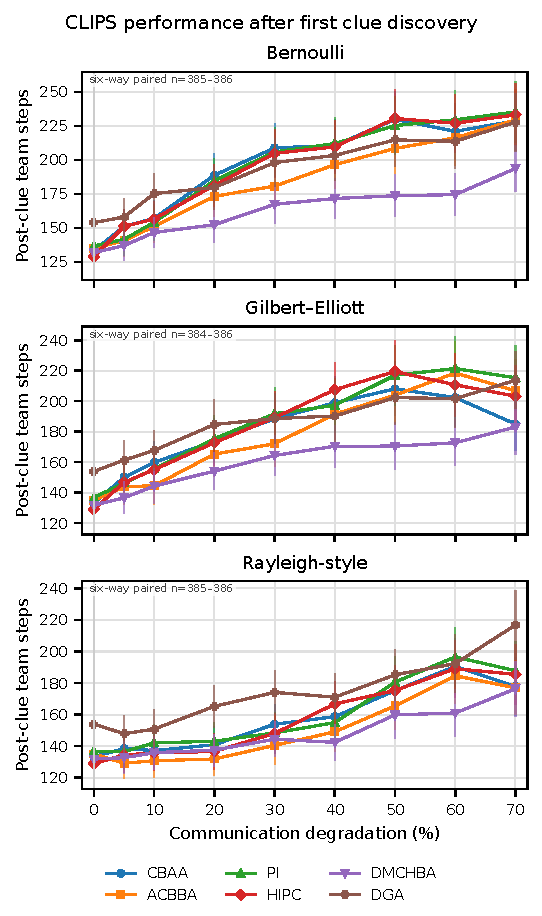
\includegraphics[width=\columnwidth]{results/analysis/figures/clips_post_clue_steps_final.pdf}
  \caption{Clue-Informed Probabilistic Search (CLIPS) performance after first clue discovery. Points are six-algorithm-paired means of \texttt{post\_clue\_steps\_to\_find}; vertical intervals are 95\% Student-$t$ confidence intervals. Each panel reports the paired sample-size range, and the ideal point is repeated at 0\% only as a common baseline.}
  \label{fig:clips-post-clue}
\end{figure}

\begin{figure*}[t]
  \centering
  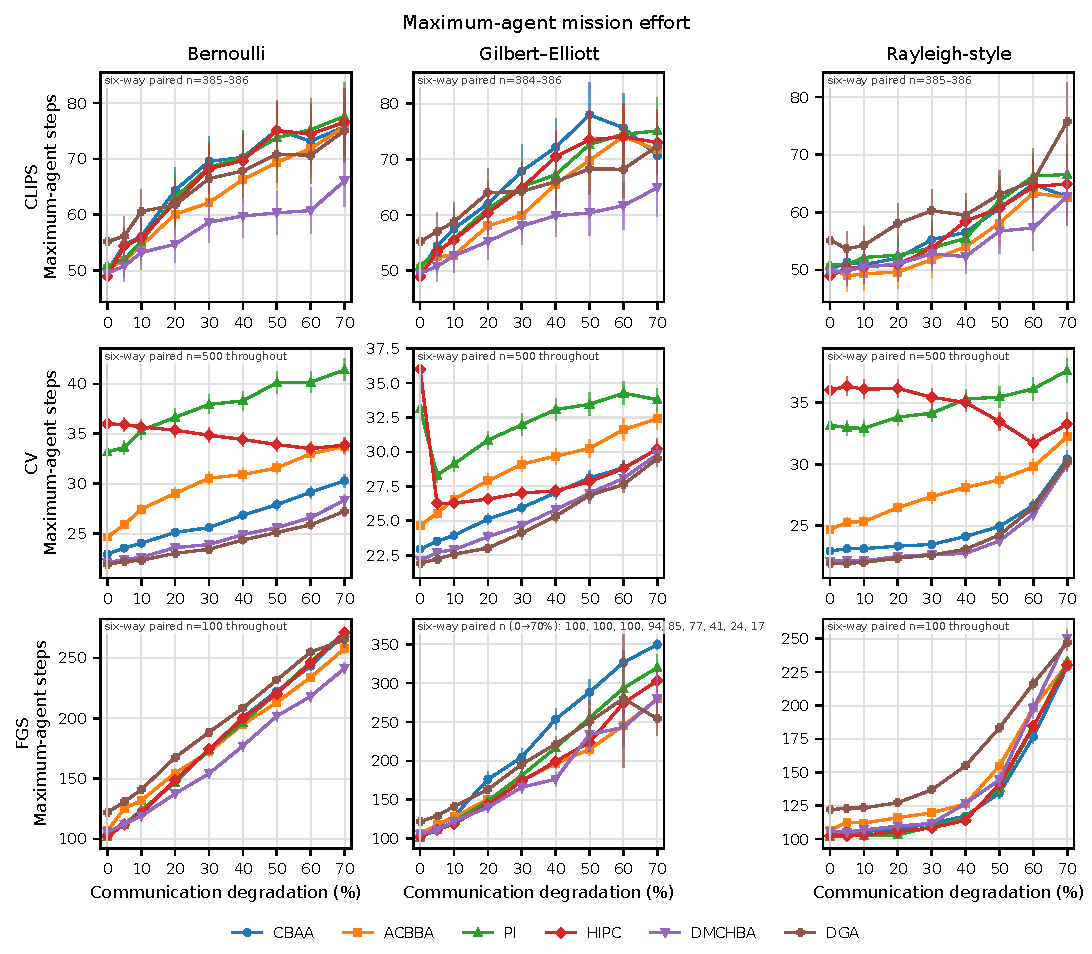
\includegraphics[width=\textwidth]{results/analysis/figures/max_agent_steps_all_missions_final.pdf}
  \caption{Maximum-agent steps for CLIPS, Collaborative Visit (CV), and Full Grid Search (FGS), separated by communication model. Points are six-algorithm-paired means with 95\% Student-$t$ confidence intervals. Printed $n$ values expose declining conditional-on-completion support for FGS under severe Gilbert--Elliott loss.}
  \label{fig:maximum-agent-steps}
\end{figure*}

\begin{figure}[t]
  \centering
  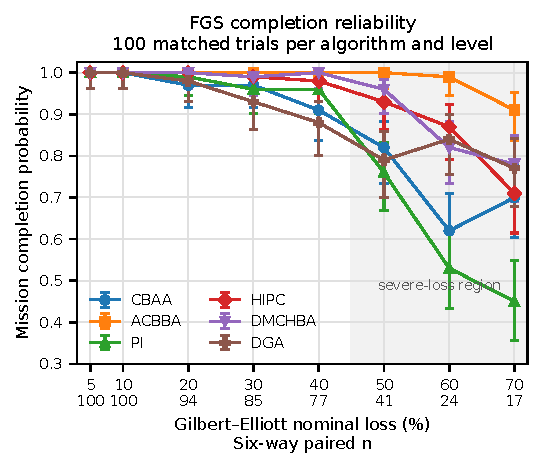
\includegraphics[width=\columnwidth]{results/analysis/figures/fgs_completion_rates_final.pdf}
  \caption{FGS mission-completion probability under the corrected Gilbert--Elliott process. Points show completion proportions over 100 matched trials per algorithm at each nominal loss level, and error bars are 95\% Wilson intervals. The second row of horizontal-axis labels reports the number of trial IDs completed by all six algorithms and therefore available for conditional continuous-metric comparison.}
  \label{fig:fgs-completion}
\end{figure}

\begin{figure}[t]
  \centering
  \includegraphics[width=\columnwidth]{results/analysis/figures/DGA_iteration.png}
  \caption{DGA generation-count sensitivity in CV under ideal and Bernoulli $p_d=0.25$ communication. Values are mean percent differences from the per-trial average over all tested DGA iteration counts. Stars mark the main-benchmark value $k=25$. The available sensitivity bundle contains no corresponding CLIPS sweep.}
  \label{fig:dga-iteration}
\end{figure}

\begin{figure*}[t]
  \centering
  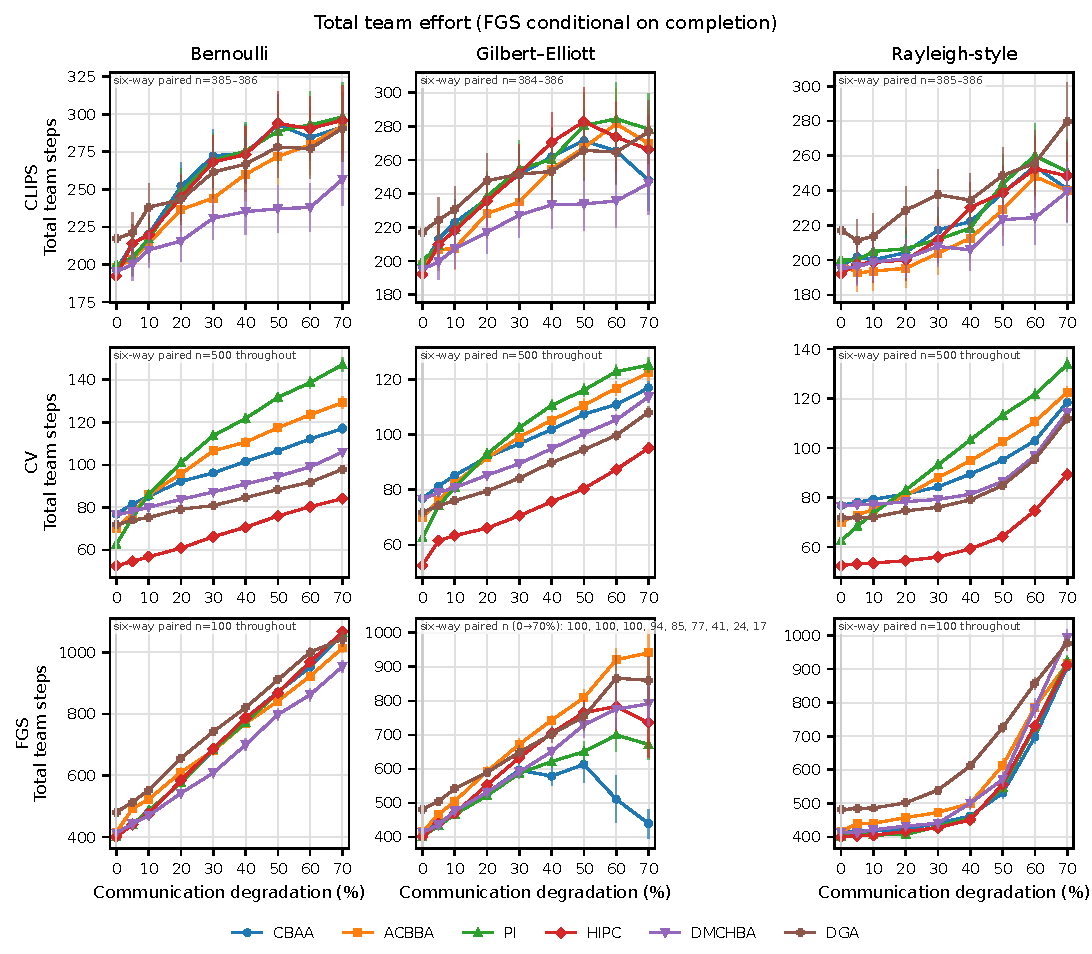
\includegraphics[width=\textwidth]{results/analysis/figures/total_team_steps.pdf}
  \caption{Total team steps by mission and communication model. Intervals represent trial uncertainty (95\% Student-$t$ confidence intervals), not ranges across degradation levels. FGS values are conditional on successful completion and use the printed six-way-paired $n$.}
  \label{fig:total-team-steps}
\end{figure*}

\begin{figure}[t]
  \centering
  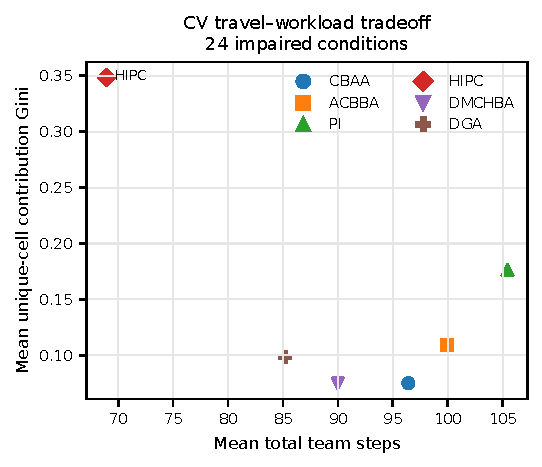
\includegraphics[width=\columnwidth]{results/analysis/figures/cv_workload_tradeoff.pdf}
  \caption{CV aggregate-travel--workload tradeoff across the 24 impaired conditions. Points show each algorithm's unweighted mean total team steps and mean unique-cell contribution Gini; the lower-left region is preferred when both total motion and workload balance matter. HIPC minimizes aggregate travel but concentrates substantially more work on a subset of robots.}
  \label{fig:cv-workload-tradeoff}
\end{figure}

\begin{figure*}[t]
  \centering
  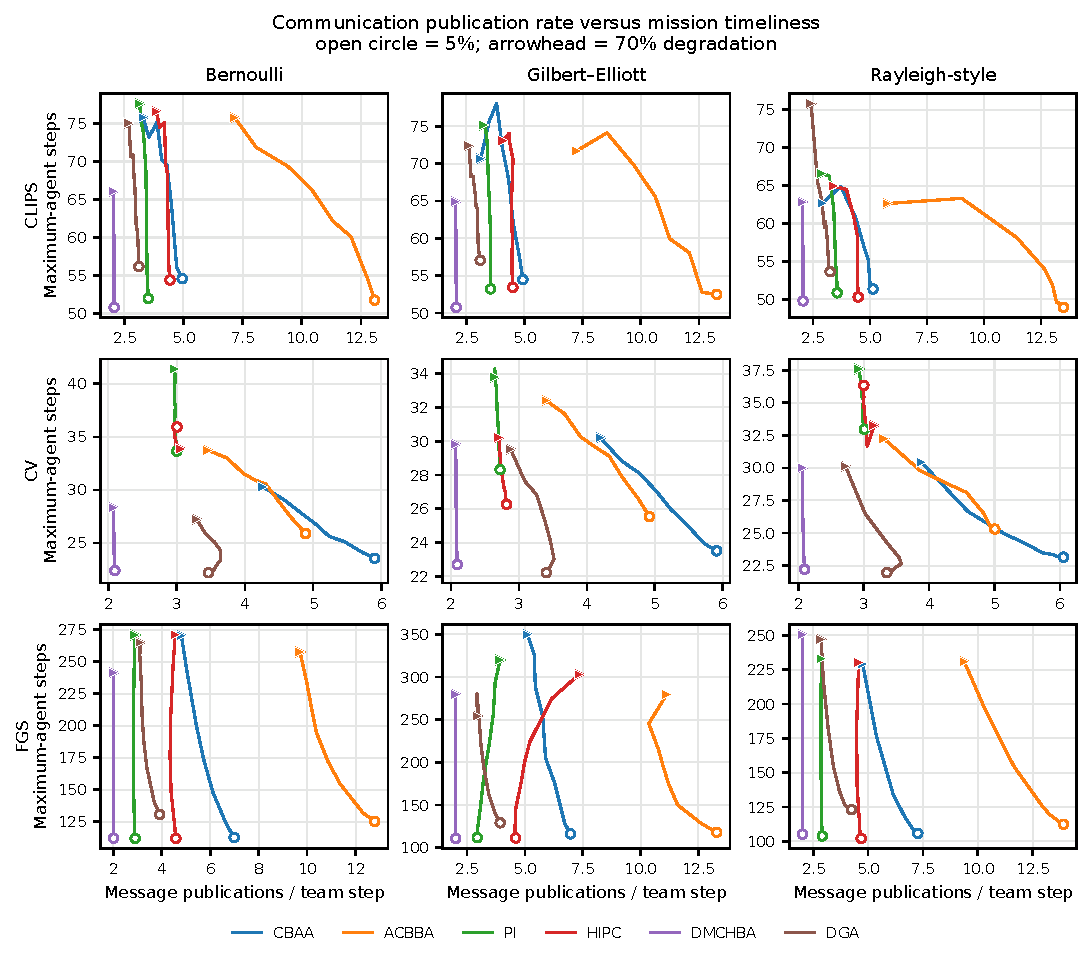
\includegraphics[width=\textwidth]{results/analysis/figures/communication_performance_tradeoff_revised.pdf}
  \caption{Communication--mission tradeoff across CLIPS, CV, and FGS. Each algorithm trajectory relates message publications per team step to absolute maximum-agent steps as nominal degradation increases from 5\% to 70\%. The lower-left region is preferred. Open circles identify 5\% and arrowheads identify 70\%; FGS points are conditional on successful completion.}
  \label{fig:communication-tradeoff}
\end{figure*}

\begin{figure*}[t]
  \centering
  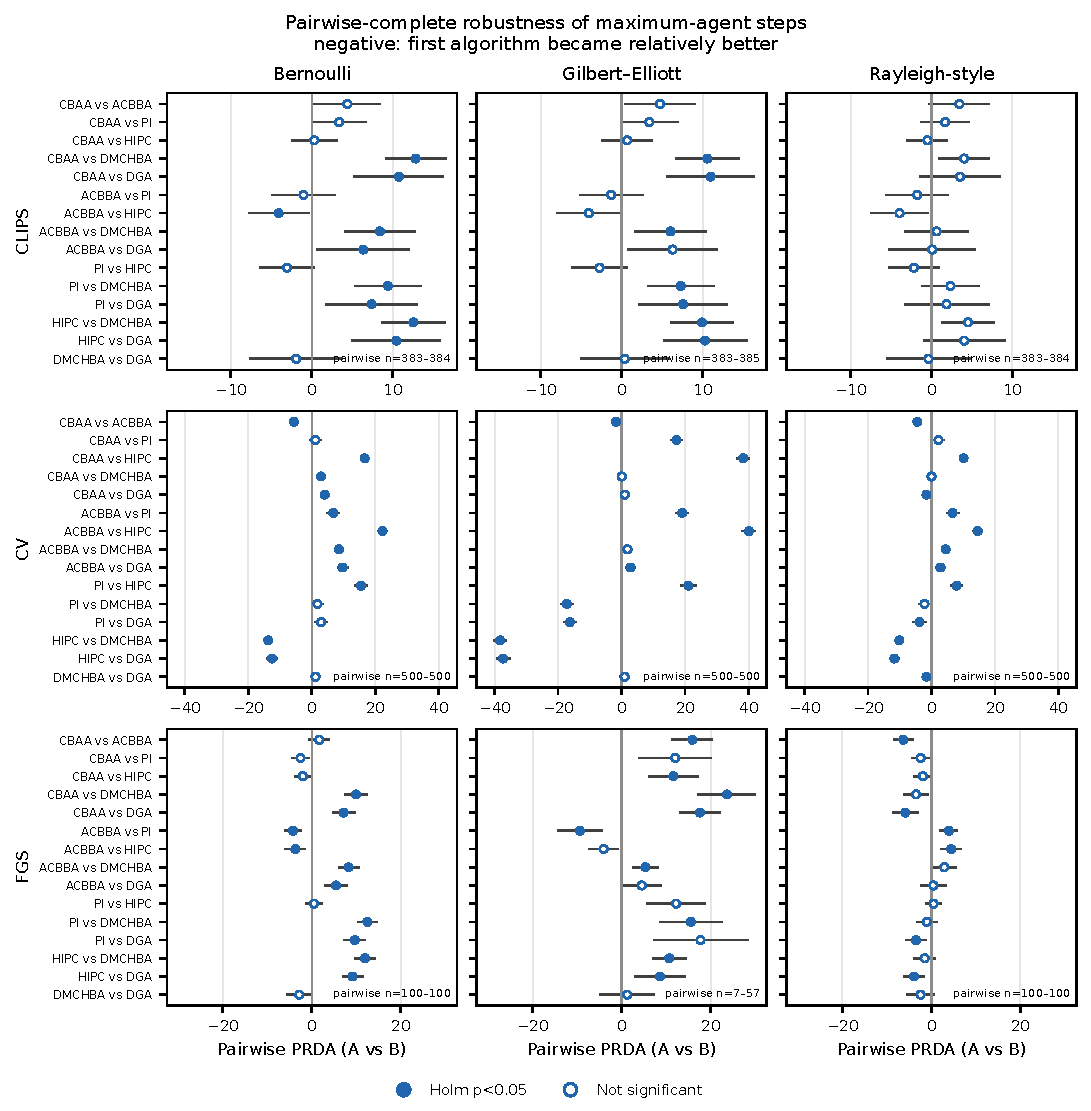
\includegraphics[width=\textwidth]{results/analysis/figures/prda_pairwise_complete_final.pdf}
  \caption{Pairwise-complete PRDA for maximum-agent steps, with communication models kept separate. Points show means with 95\% Student-$t$ confidence intervals. Negative values mean the first named algorithm became relatively better as degradation increased. Filled markers denote Holm-adjusted $p<0.05$, open markers denote nonsignificant comparisons, and panel annotations give pairwise-complete $n$ ranges.}
  \label{fig:pairwise-prda}
\end{figure*}

\begin{figure*}[t]
  \centering
  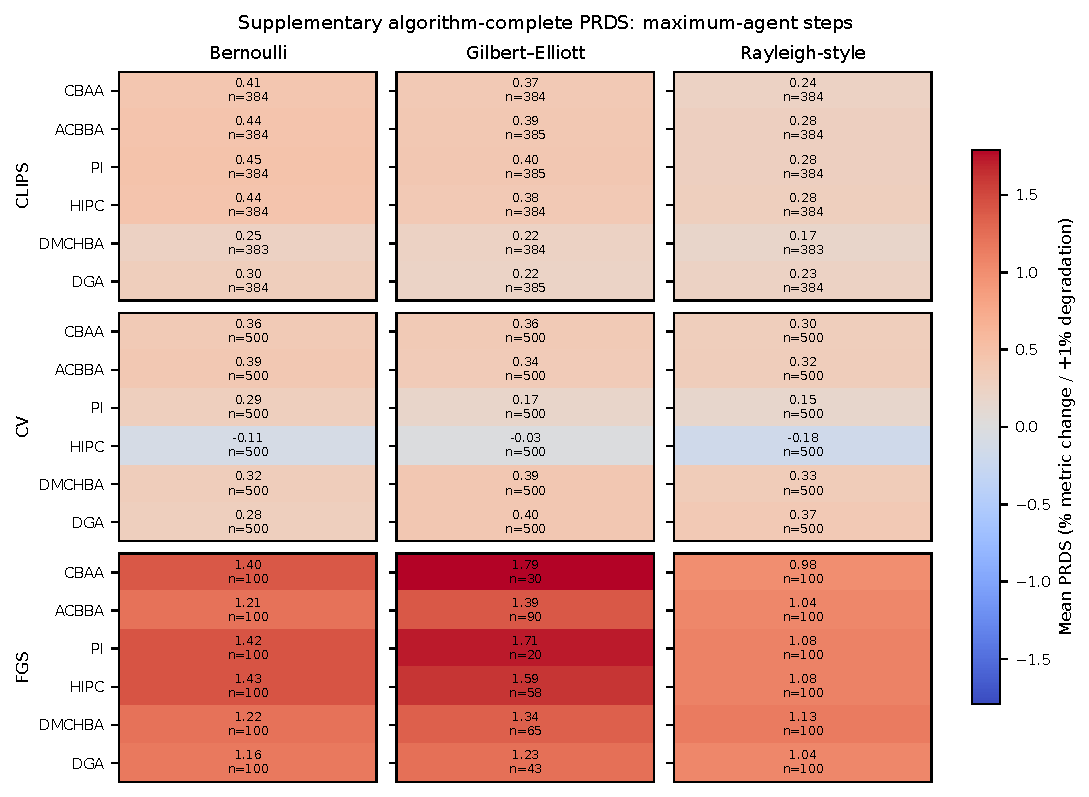
\includegraphics[width=\textwidth]{results/analysis/figures/prds_supplement.pdf}
  \caption{Supplementary algorithm-complete PRDS for maximum-agent steps. Communication models are not averaged; each cell reports the mean PRDS and eligible algorithm-specific trajectory $n$.}
  \label{fig:prds-supplement}
\end{figure*}

\begin{figure}[t]
  \centering
  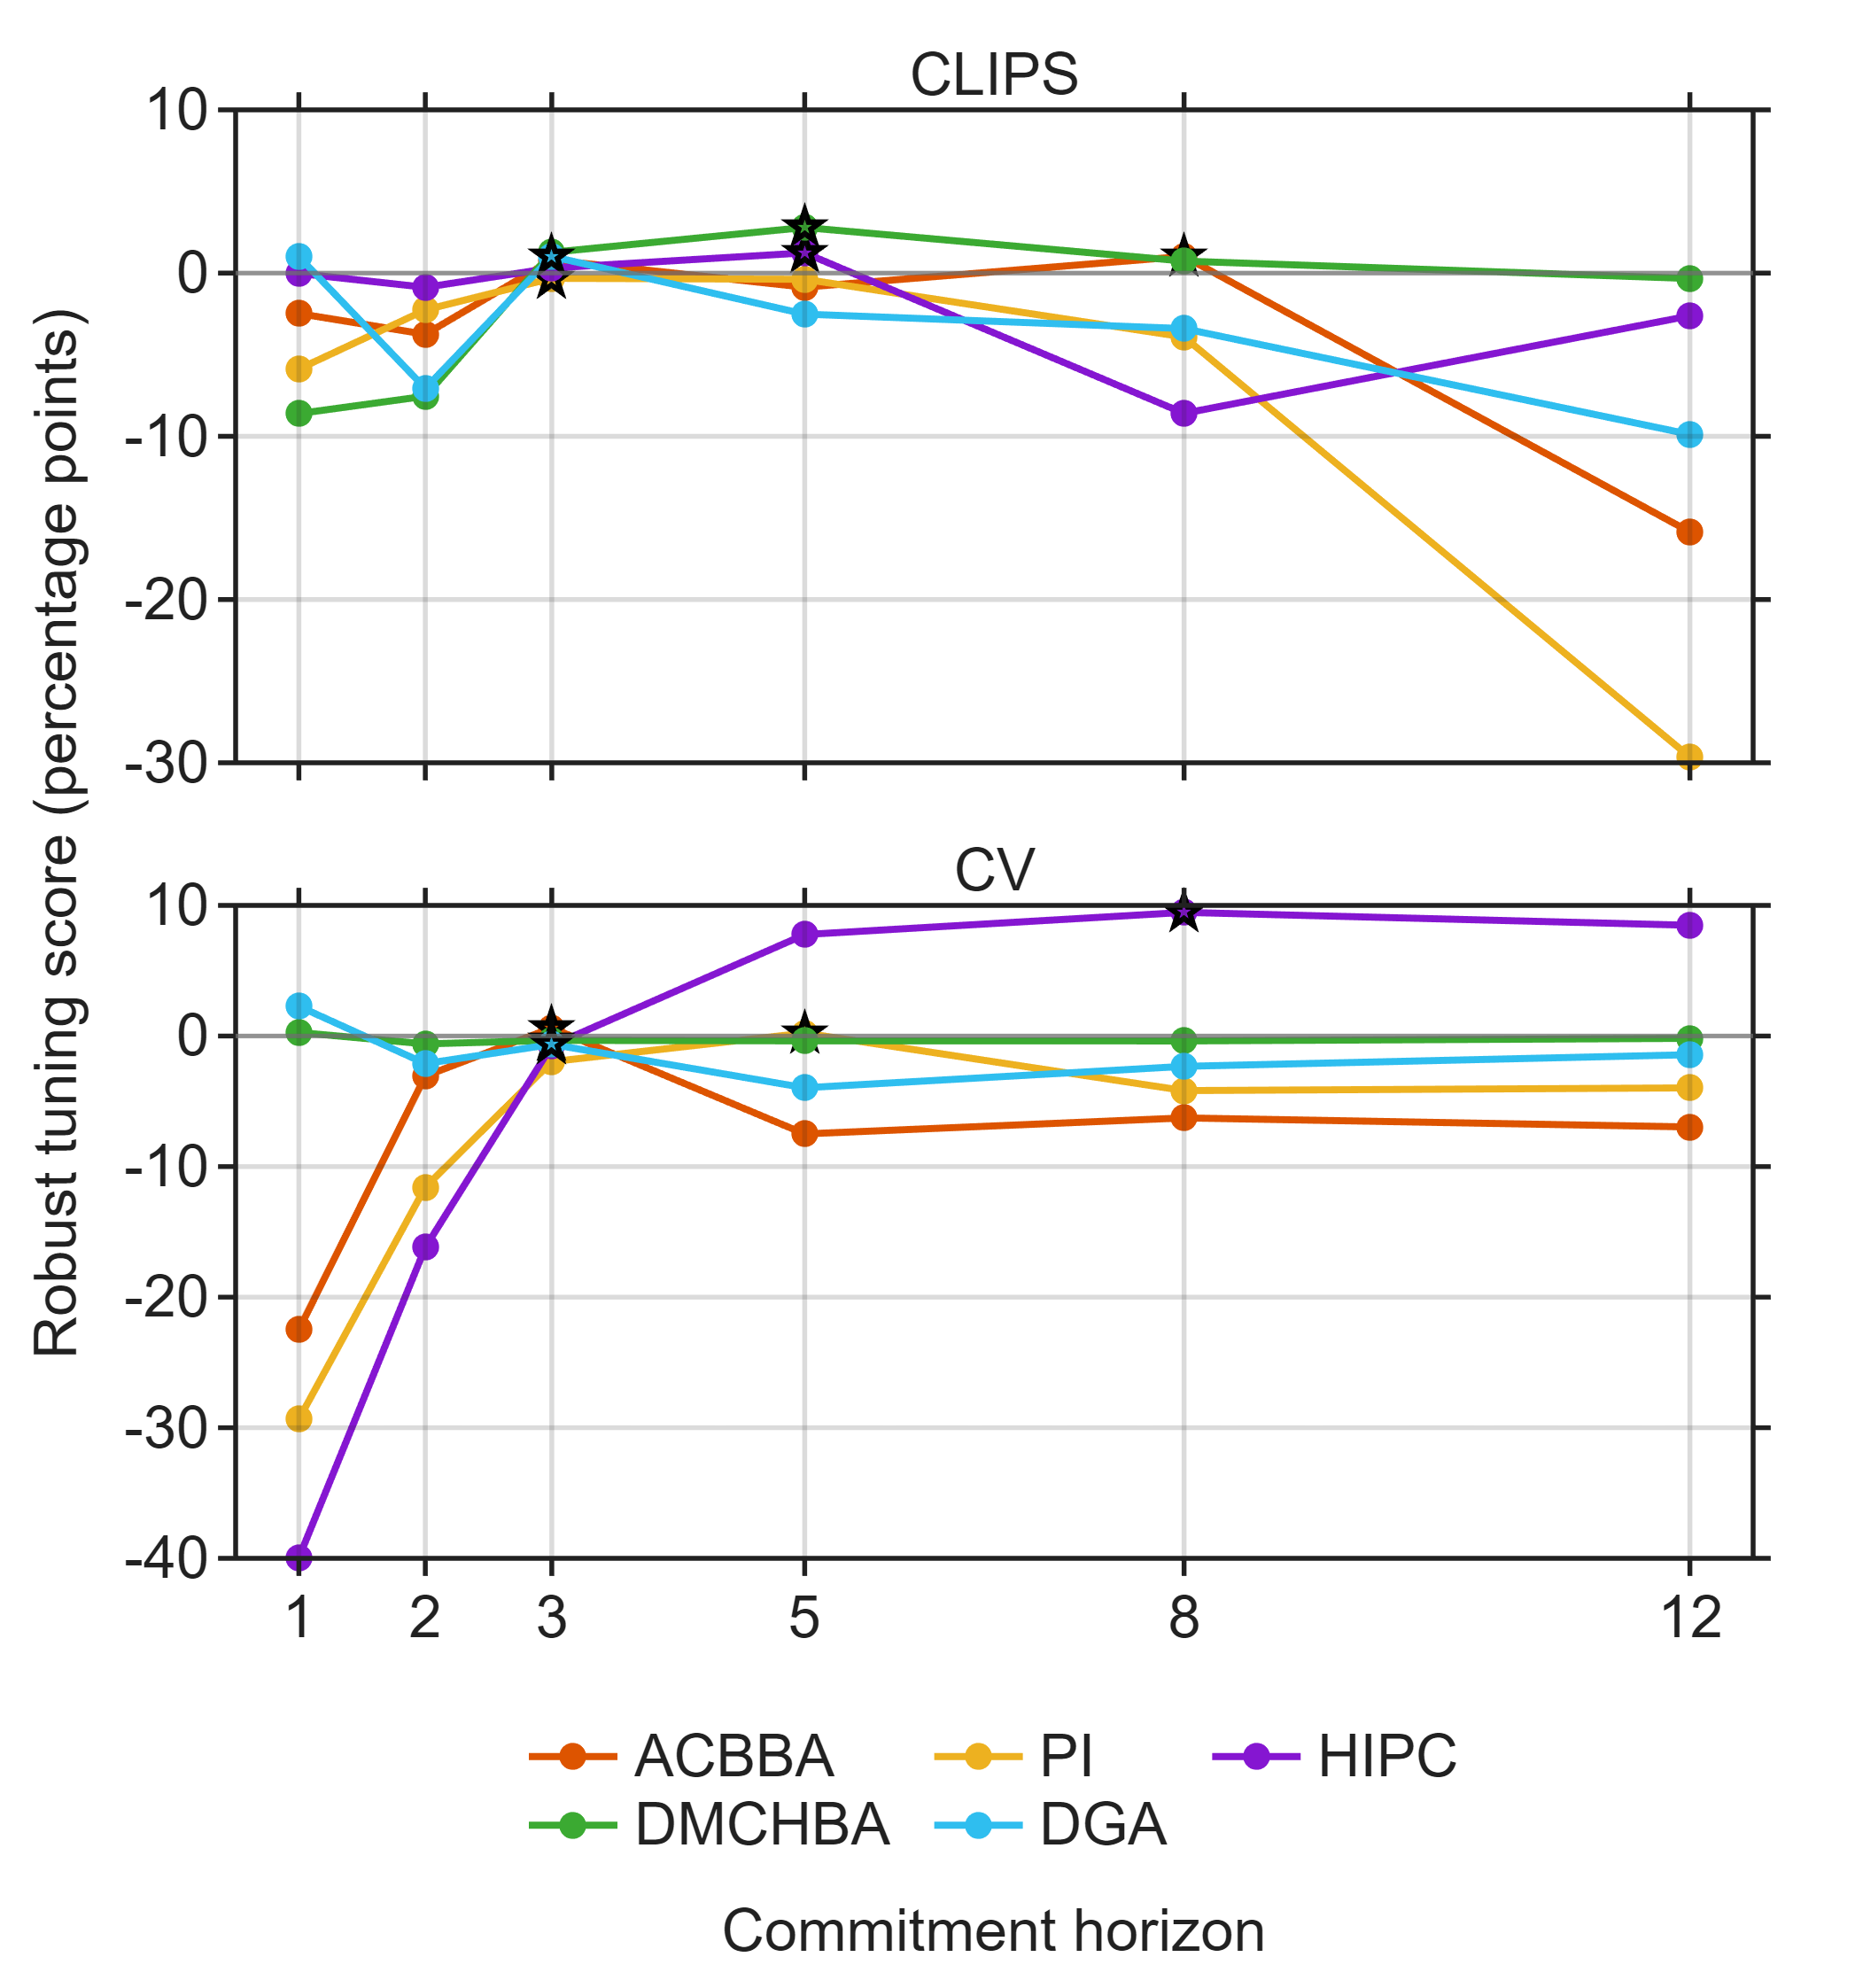
\includegraphics[width=\columnwidth]{results/analysis/figures/horizon_tuning.png}
  \caption{Commitment-horizon sensitivity for CV, CLIPS, and FGS. Within each mission, algorithm, and trial, the paired baseline is the mean metric over all tested horizons and both communication settings; plotted values are metric-minus-baseline means. Solid lines denote ideal communication, dotted lines Bernoulli loss probability 0.25, and stars mark the selected main-benchmark horizon for each algorithm and mission.}
  \label{fig:horizon-tuning}
\end{figure}
